\section{Singapore --- Electronic Road Pricing (ERP)}

\subsection{History}

Over time, ALS became hard to administer as Singaporean authorities priced vehicles more precisely. \citet[p. 4]{Chin2009} describes ALS once multiple charging periods and vehicle classes had been added: ``There were 16 different types of licences in use at its peak, and much concentration by the enforcement officers was required to ensure that they identified them correctly.'' The license system also precluded charging for each entry or varying prices in small time increments.

Therefore, in 1990 Singapore solicited bids for a wireless system which would be called, like Hong Kong's, Electronic Road Pricing (ERP). Wary of the privacy concerns that had helped sink Hong Kong's ERP, authorities chose a ``smart card'' system, whereby a roadside beacon tells a device on the vehicle to deduct money from a stored-value card \citep{PhangToh1997,Chin2009}. This setup obviates keeping records of every vehicle's movements. In 1995, the contract for the system was awarded to a consortium led by Phillips Singapore, and after extensive field trials and publicity, ERP commenced full operation on September 1st, 1998.

\subsection{Design}

\citet{Menon2004} describes ERP as having three components.

\begin{itemize}
\item In-vehicle Unit (IU), an electronic device that sits on vehicles' dashboards or handlebars. The IU has a slot for a ``CashCard'' that the user can load up with money at various establishments---similar to transit touch cards in wide use today. Since March 2015, a sevice called vCashCard allows drivers to pay with debit or credit without having a physical CashCard in the IU. (http://www.straitstimes.com/singapore/transport/virtual-cashcard-aims-to-solve-erp-woes) There are IU's for each of six vehicle classes (see Figure \ref{fig:singapore-IUs}), because the toll charged to a vehicle is a multiple of its ``Passenger Car Unit'' (PCU), an index of size (see Table \ref{tab:passenger-car-units}). 

\item Gantries, metal archways positioned in pairs over the road at tolling sites. When a vehicle passes below, the first gantry tells the vehicle's IU to charge appropriately. An optical sensor on the second gantry confirms the vehicle type matches the IU. In the event of a transaction error, a camera on the first gantry captures the rear number plate. 

\item The central control system, which verifies charges and issues notices and fines when there is a violation or error.
\end{itemize}

\begin{table}
	\begin{tabular}{|c|c|}
		\hline 
		PCU's & Vehicles\tabularnewline                              
		\hline 
		\hline 
		0.5   & motorcycles\tabularnewline                           
		\hline 
		1     & cars, taxis, light goods vehicles\tabularnewline     
		\hline 
		1.5   & heavy goods vehicles/small buses\tabularnewline      
		\hline 
		2     & very heavy goods vehicles/large buses\tabularnewline 
		\hline 
	\end{tabular}
	
	\caption{
	Passenger Car Units (PCU's) for ERP. Vehicle charges are weighted by the PCU number---e.g., a very heavy goods vehicle pays four times what a motorcycle does. \citep{LTA2016} 
	}
	\label{tab:passenger-car-units}
\end{table}

Tolls vary substantially over the day. Figure \ref{fig:singapore-toll-schedule} illustrates a weekday toll schedule to enter the main part of the CBD in different years. For the first five years of ERP, tolls changed only at half-hour intervals. But since February 2003, whenever tolls change by more than S\$1, there is a five-minute interval in which tolls rise or fall by half the amount of the change, in order to discourage cars from slowing down or speeding up when tolls are about to change \citep{Menon2004}. The Land Transport Authority (LTA) updates prices quarterly to maintain speeds of 45-65kph on expressways and 20-30 kph on roads in the CBD.
	
\begin{figure}
	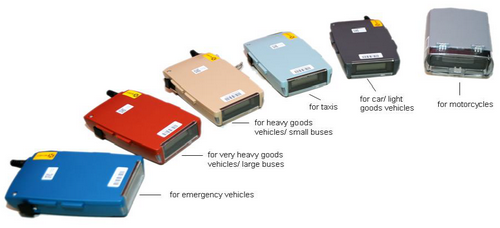
\includegraphics[width=4in]{../img/singapore-IUs.jpg}
	\caption{ERP In-vehicle units \citep{LTA2016}}
	\label{fig:singapore-IUs}
\end{figure}

% \begin{figure}
% 	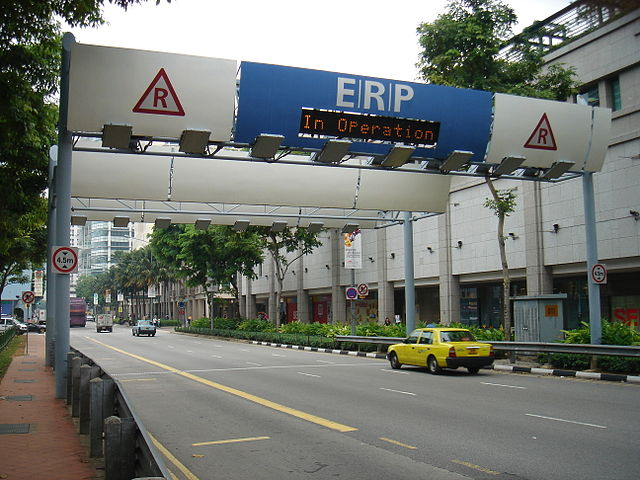
\includegraphics[width=4in]{../img/singapore-gantry.jpeg}
% 	\caption{ERP gantry \citep{LTA2016}}
% 	\label{fig:singapore-gantry}
% \end{figure}


\begin{figure}
	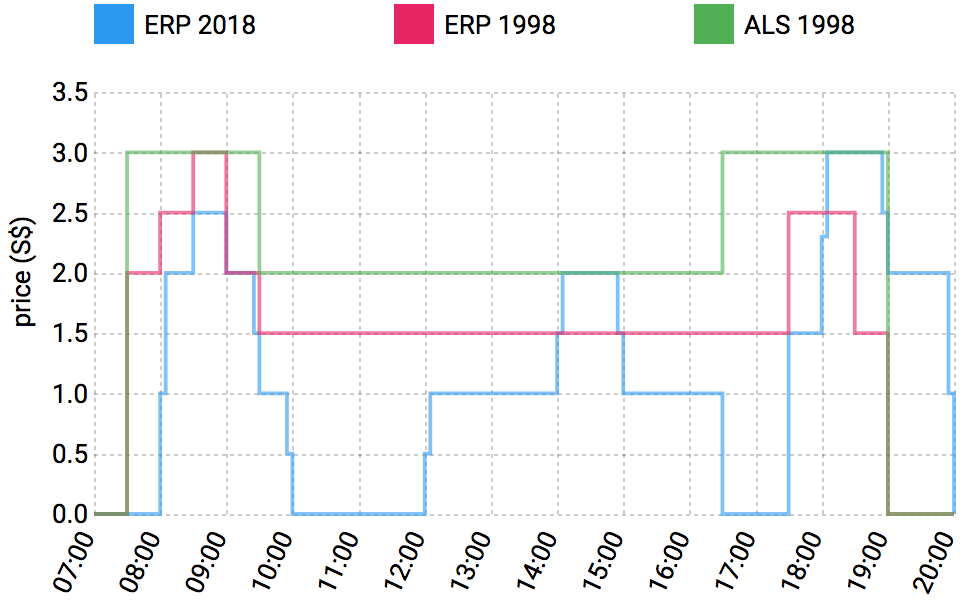
\includegraphics[width=1\textwidth]{../img/singapore-prices.png}
	\caption{Singapore prices for different years. The schedule becomes more variable as years pass. }
	\label{fig:singapore-toll-schedule}
\end{figure}

The substantial changes to ERP have been spatial \citep{Chin2009,LTA2018}. ERP started in 1998 with 33 tolling sites replacing the extant ALS and Road Pricing Scheme tolling sites. Since then, the scheme has been greatly expanded. The DCP element of the scheme consists of 39  tolling sites enclosing three contiguous sub-cordons in the CBD. One, the Orchard Road Cordon, contains shopping areas and is thus unpriced on weekday mornings. The other two---the Bugis-Marina Centre Cordon and the Shenton Way-Chinatown Cordon---contain offices and thus operate all day during the weekdays. In the morning, traveling between these two sub-cordons is free---effectively making a single CBD cordon---but there is a small charge to do so between 6 and 8 PM, in order to limit intra-CBD congestion. There are also 54 tolling sites further out from the CBD to control traffic on expressways and arterials. 
% \footnote{https://www.onemotoring.com.sg/content/onemotoring/en/on\_the\_roads/ERP_Rates/\_jcr\_content/main\_par/expandcollapse\_935498777/par/expandcollapse/par/download/file.res/Cars\%20-\%206\%20Nov\%202017.pdf}

\subsection{Results}

The transition to ERP was not as thoroughly documented as the launch of ALS. One significant effect is that entries to the CBD fell by about 15\%, largely due to a decline in repeat trips by the same vehicle \citep{Menon2000}. Since ALS permitted unlimited same-day entries, under ALS about 23\% of trips had been repeat trips---e.g., office workers using cars for lunches and meetings in the middle of the day \citep[p. 23]{Chin2009}. \citet{Olszewski2005} conclude, using data from before and after ERP, that the LTA's charging structure has done a good job controlling congestion and spreading traffic flow over the peaks.

\subsection{Finances}

Implementation cost S\$197 million in 1998, of which S\$100 million paid for IU's (since the launch this expensive is incurred by the vehicle owner) and S\$97 million to build out the infrastructure \citep{Santos2004}. Annual operating costs have measured about 20-30 percent of revenues \citep{Chin2009}.

ERP revenues in 1999 were S\$68 million---down a third from the S\$100 million earned by ALS and the Road Pricing Scheme in 1998 \cite[p. 34]{Goh2002}. Revenues fell because ERP prices were lower than the ALS charge, which, combined with the significant investment cost and higher operating cost, makes it clear that the switch to ERP was not motivated by revenue concerns. In 2012 ERP revenues were S\$159 million \citep{Chen2012}. Revenue is not hypothecated but rather flows into the governent's general fund.

